\documentclass[11pt]{exam}
\RequirePackage{amssymb, amsfonts, amsmath, latexsym, verbatim, xspace, setspace}
\RequirePackage{tikz, pgflibraryplotmarks}

\usepackage[margin=1in]{geometry}
\usepackage[utf8]{inputenc}


% Here's where you edit the Class, Exam, Date, etc.
\newcommand{\class}{Seminario de tecnología}
\newcommand{\examnum}{Examen Parcial 2}
\newcommand{\term}{2 Cuatrimestre, 2014}
\newcommand{\examdate}{17/10/14}
\newcommand{\timelimit}{120 minutos}

% For an exam, single spacing is most appropriate
\singlespacing
% \onehalfspacing
% \doublespacing

% For an exam, we generally want to turn off paragraph indentation
\parindent 0ex

\begin{document} 

% These commands set up the running header on the top of the exam pages
\pagestyle{head}
\firstpageheader{}{}{}
\runningheader{\class}{\examnum\ - Pagina \thepage\ de \numpages}{\examdate}
\runningheadrule

\begin{flushright}
\begin{tabular}{p{2.8in} r l}
\textbf{\class} & \textbf{Nombre:} & \makebox[2in]{\hrulefill}\\
\textbf{\term} &&\\
\textbf{\examnum} &&\\
\textbf{\examdate} &&\\
\textbf{Tiempo: \timelimit}
\end{tabular}\\
\end{flushright}
\rule[1ex]{\textwidth}{.1pt}


Este examen consta de \numpages\ paginas y \numquestions\ preguntas. Verifique que tiene todas las hojas necesarias. Las preguntas se responden en la misma hoja del examen.\\

El examen se puede realizar a libro abierto y esta permitido el uso de calculadora si es requerido. Se puede utilizar el contenido del primer  examen como referencia. Se puede utilizar computadora.\\

Las siguientes reglas aplican para la aprobación del examen:\\

\begin{minipage}[t]{3.7in}
\vspace{0pt}
\begin{itemize}
\item Escritura de todas las \textbf{respuestas en tinta, sin excepción}.-
\item \textbf{Se requiere un mínimo de 10 puntos} para la aprobación del examen.-
\item Justificar sus respuestas, en caso de ser necesario, con diagramas o ejemplos claro.-
\item Lea todo el examen antes de comenzar a responder. Algunas preguntas guardan relación con otras y pueden servir de ayuda.-
\end{itemize}

No escriba en la tabla de la derecha.\\
\\
\textbf{Mucha suerte! :)}

\end{minipage}
\hfill
\begin{minipage}[t]{2.3in}
\vspace{0pt}
%\cellwidth{3em}
\gradetablestretch{2}
\vqword{Pregunta}
\addpoints % required here by exam.cls, even though questions haven't started yet.	
\gradetable[v]%[pages]  % Use [pages] to have grading table by page instead of question

\end{minipage}
\newpage % End of cover page

%%%%%%%%%%%%%%%%%%%%%%%%%%%%%%%%%%%%%%%%%%%%%%%%%%%%%%%%%%%%%%%%%%%%%%%%%%%%%%%%%%%%%
%
% See http://www-math.mit.edu/~psh/#ExamCls for full documentation, but the questions
% below give an idea of how to write questions [with parts] and have the points
% tracked automatically on the cover page.
%
%
%%%%%%%%%%%%%%%%%%%%%%%%%%%%%%%%%%%%%%%%%%%%%%%%%%%%%%%%%%%%%%%%%%%%%%%%%%%%%%%%%%%%%

\begin{questions}

% Pregunta 1
\addpoints
\question[2] Defina con sus palabras el concepto de IoT (Internet of Things).
\vspace{4.5in}
% Pregunta 2
\addpoints
\question[2] Indique cual de estas organizaciones define los estándares para las arquitecturas de redes de sensores.
\begin{itemize}
\item IEEE
\item ITU
\item ACM
\end{itemize}

% Pregunta 3
\addpoints
\question[2] Indique cual/es de los siguientes items no formna parte de una arquitectura de IoT.
\begin{itemize}
\item Backend DB
\item Sensor/es varios
\item Modulo de conectividad (Ethernet, RF, WiFy, etc.)
\item CRM
\item BI
\end{itemize}
\newpage
% Basic question
\addpoints
\question[2] Cuando se leen señales analógicas, utilizando un microprocesador, se hace uso de un componente especifico, marque la opción correcta:
\begin{itemize}
\item ADC
\item ALU
\item Timer
\item PWM
\end{itemize}

\addpoints
\question[3] Se debe muestrear una señal analógica de una Foto resistencia (utilizada para medir presencia de luz) conectada a un puerto, donde la señal varia entre 0 y 5 Volts. Se dispone de un microprocesador que tiene un ADC (conversor analógico digital) de 8 bits de resolución ($2^{3bits}=1024$). Indique el valor en Volts de cada nivel muestreado:
\begin{itemize}
\item 1
\item 0.5
\item 0.1
\item Ninguna
\end{itemize}

Recuerde: 
$$V_{muestra} = \frac{Voltage}{Cantidad-de-muestras}$$


\addpoints
\question[3] Describa la importancia de IPv6 en el desarrollo de IoT.
\vspace{2in}

\addpoints
\question[2] Las bases de datos son una parte fundamental de los sistemas de sensores. Indique que tipo de base utilizaría para guardar solamente datos históricos de un sensor. Justifique.
\begin{itemize}
\item No relacional (MongoDB)
\item Relacional (MySQL)
\item Ninguna
\end{itemize}

\newpage
\addpoints
\question[4] A partir del siguiente esquema, identifique las "capas" de una arquitectura IoT y sus componentes. Tenga en cuenta las capas descritas y relacione con el prototipo desarrollado en el primer examen. Describa brevemente que medios de enlace utilizaría para conectar el prototipo a Internet y como plantearía el backend (almacenamiento) y frontend (management).\\

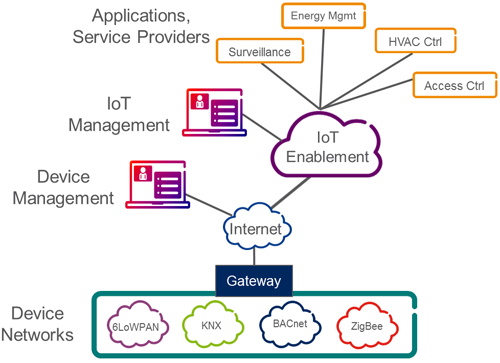
\includegraphics[scale=0.7]{iotarch.png} 






















\end{questions}
\end{document}